\subsection*{Analysis Outliers Packages: Stable Trend}
\label{sec:analysisPackageSizeStable}

\begin{figure}[H]
    \centering
    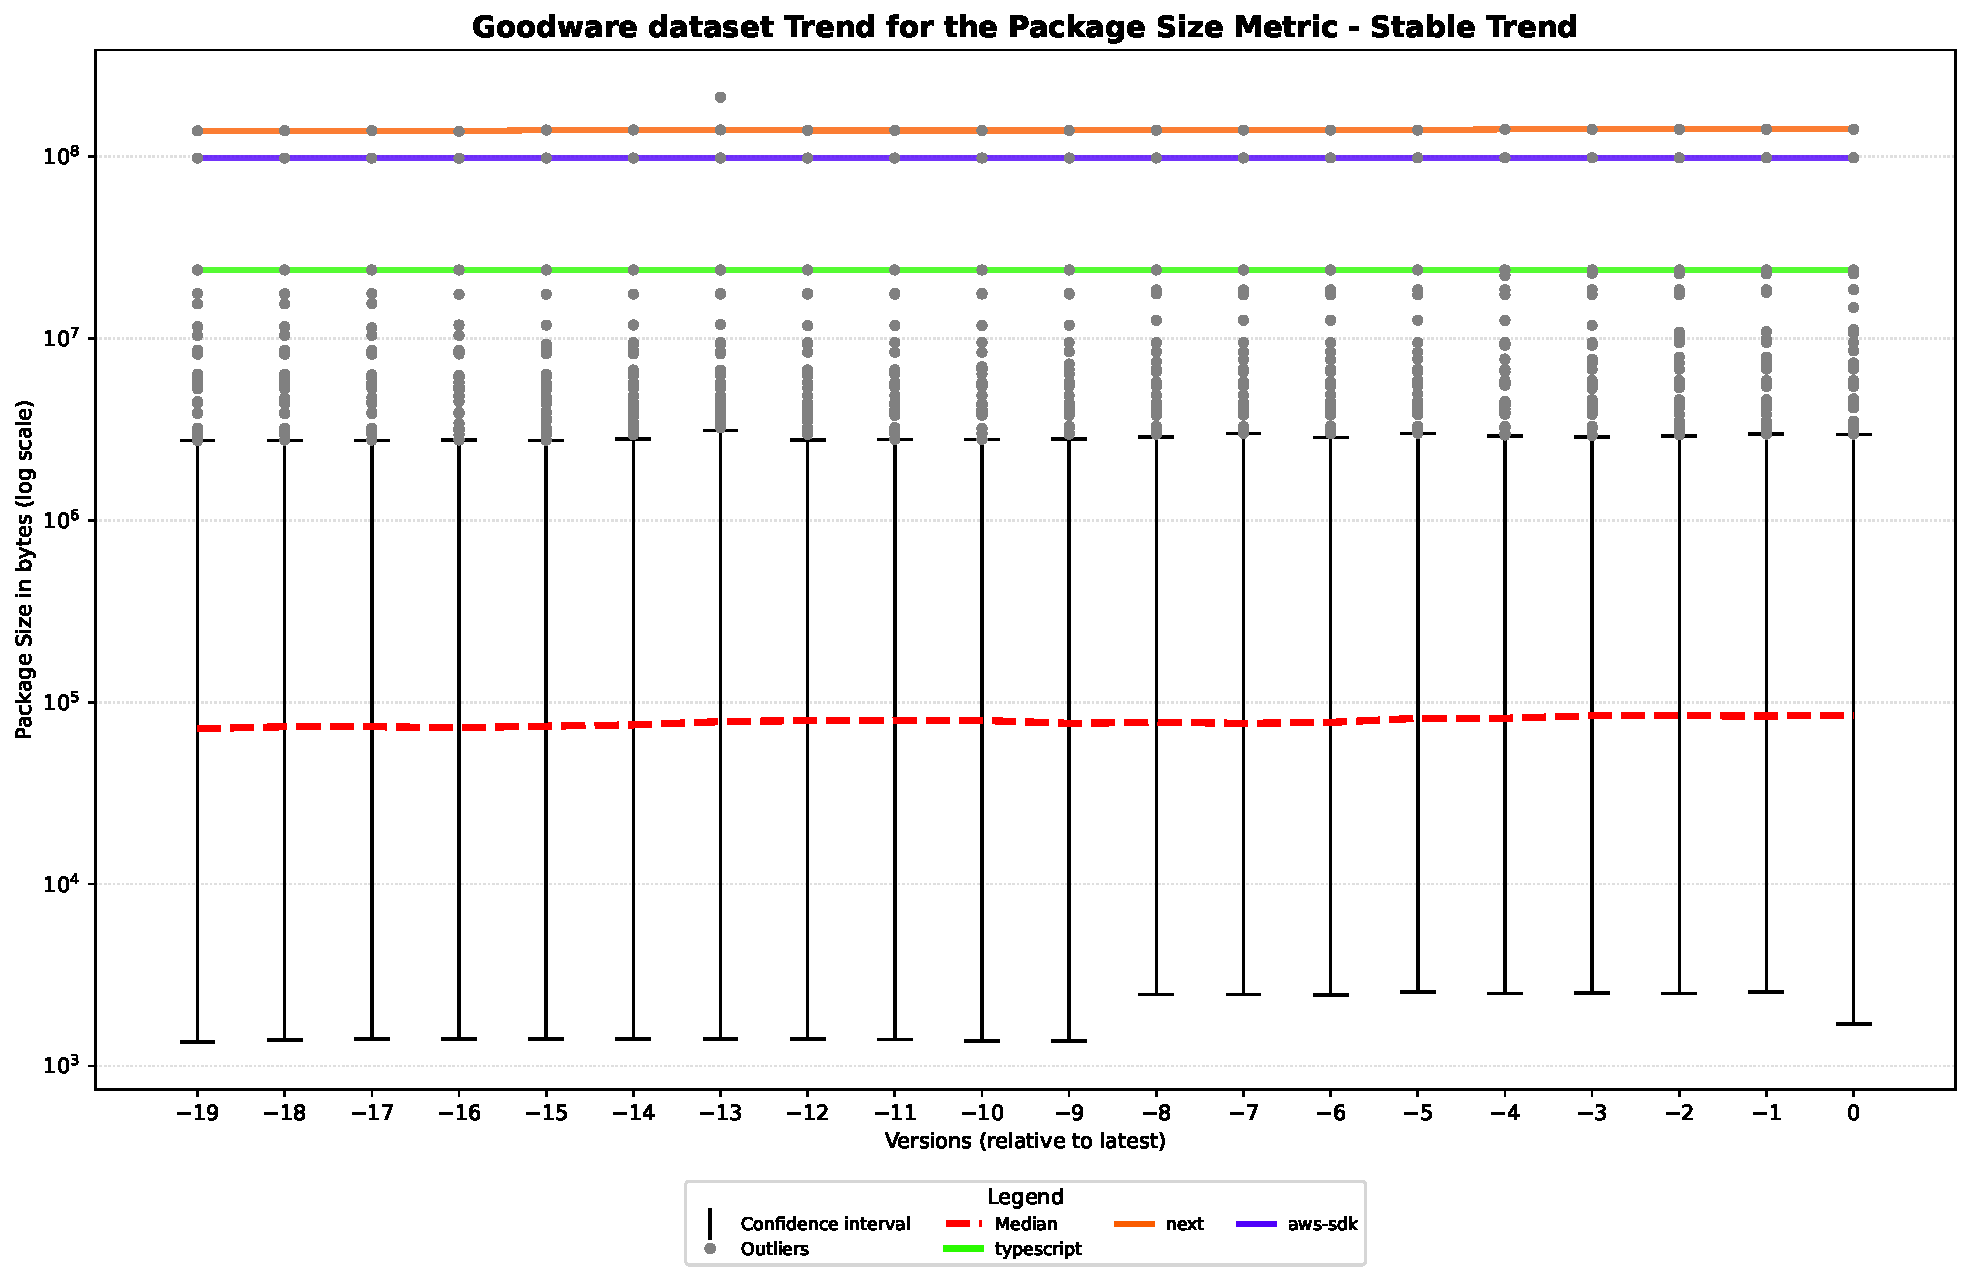
\includegraphics[width=\textwidth]{metrics/packageSize/PS_plot1_Stable_Trend.pdf}
    \caption{Outliers package Stable Trend for the Package Size Metric in Goodware dataset}
    \label{fig:fig1PackageSizeStable}
\end{figure}

The remaining three highlighted packages had outlier values that remained constant across all 20 versions, without significant increases or decreases.
The packages exhibiting this trend are: \texttt{next}, \texttt{aws-sdk} and \texttt{typescript}.

\begin{itemize}

    \item \textbf{next:} This package is a React full-stack framework~\cite{next}.
    Represented by the solid orange line in \cref{fig:fig1PackageSizeStable}, the package has a size of 140 MB across all versions.
    It is the most extreme outlier in all versions except in version -13, 
    where it was surpassed by \texttt{moment-timezone}, as seen in \cref{sec:analysisPackageSizeIncreasing}.

    \item \textbf{aws-sdk:} This is the official package for interacting with \ac{AWS} cloud services~\cite{aws-sdk}.
    Represented by the solid purple line in \cref{fig:fig1PackageSizeStable}, the package has a size of 98 MB across all versions.

    \item \textbf{typescript:} This package provides the official compiler and toolset for the TypeScript language~\cite{typescript}.
    Represented by the solid green line in \cref{fig:fig1PackageSizeStable}, it maintains a constant size of 23.7 MB across all versions.

\end{itemize}


\subsection{Comparison with Malware Dataset}
\label{sec:analysisPackageSizeComparisonMalware}

We analyzed when this metric is effective for detecting these four attacks (described in \cref{ch:AnalysisRecentAttacks}) and when it is not indicative.
To do so, we used a specific figure for each attack, \cref{fig:fig2PackageSizeAttackA}, \cref{fig:fig2PackageSizeAttackB},
\cref{fig:fig2PackageSizeAttackC} and \cref{fig:fig2PackageSizeAttackD}, as explained in \cref{sec:Figure2}.

\subsection*{Attack A: Malicious Windows DLL}
\label{sec:analysisPackageSizeAttackA}

\begin{figure}[H]
    \centering
    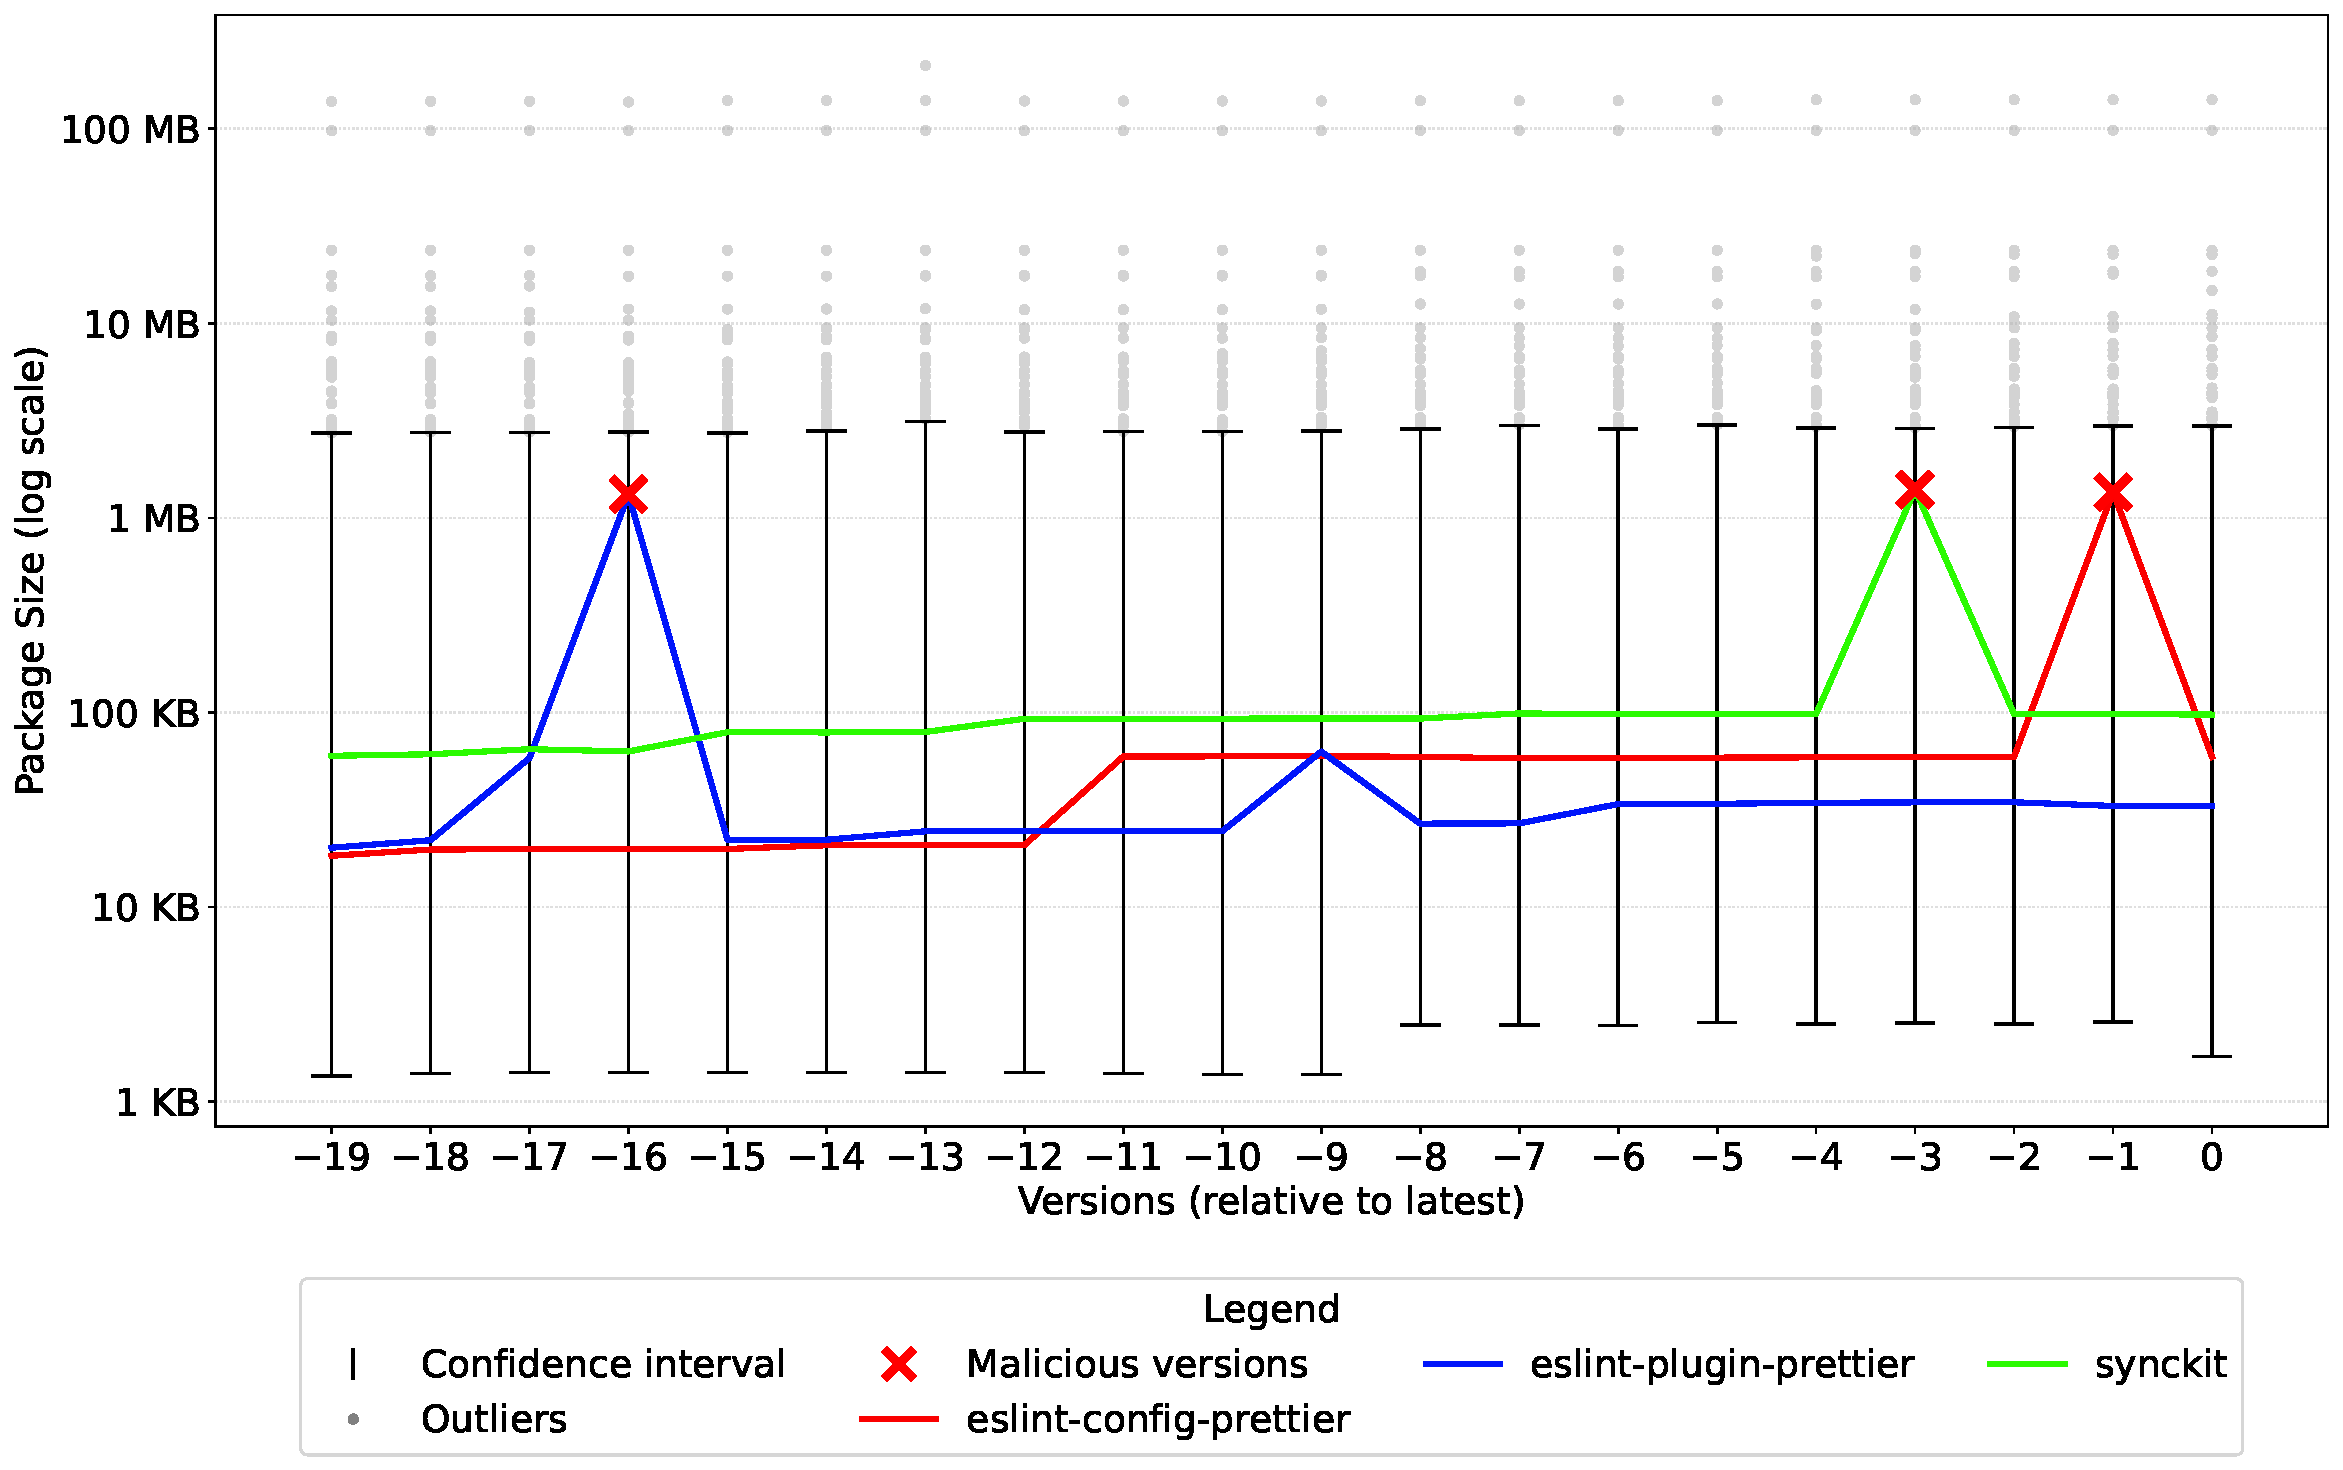
\includegraphics[width=\textwidth]{metrics/packageSize/PS_plot2single_AttackA.pdf}
    \caption{Comparison with Malware Dataset Package Size Metric for Attack A}
    \label{fig:fig2PackageSizeAttackA}
\end{figure}

In attack A (\cref{sec:attackA}), the attacker inserted a malicious \ac{DLL} weighing 1.2 MB into the tarball.
As shown in \cref{fig:fig2PackageSizeAttackA},
the compromised versions of the three packages from the Malware dataset affected by this attack do not reach outlier values.
Consequently, the metric is not able to detect this specific attacks and results as not indicative.

\subsection*{Attack B: Crypto attack}
\label{sec:analysisPackageSizeAttackB}

\begin{figure}[H]
    \centering
    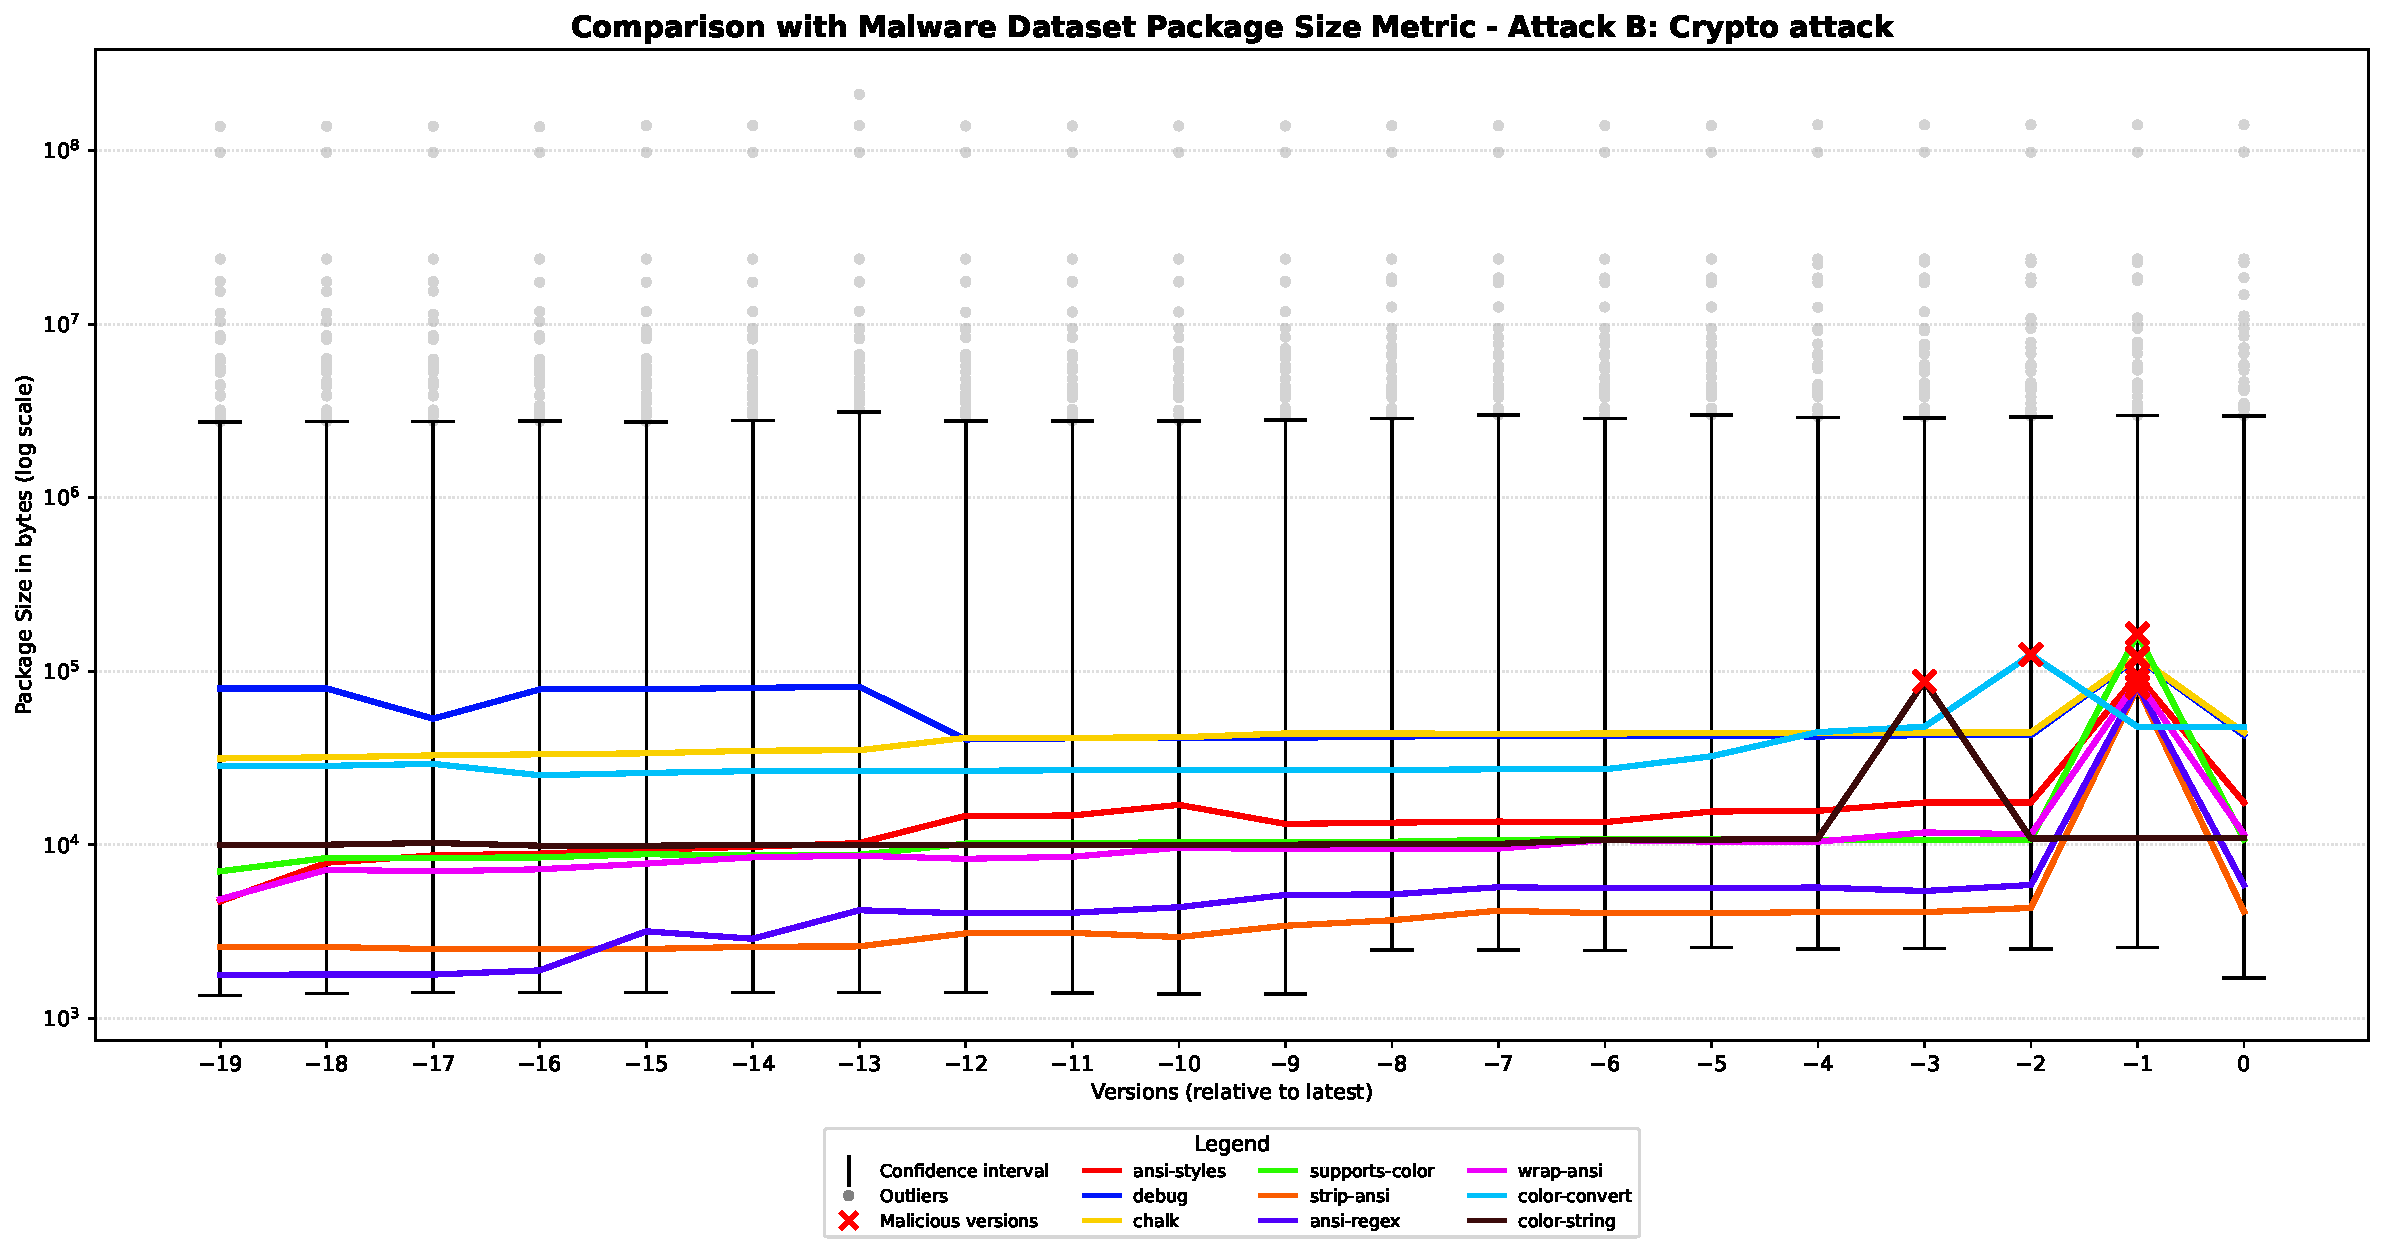
\includegraphics[width=\textwidth]{metrics/packageSize/PS_plot2single_AttackB.pdf}
    \caption{Comparison with Malware Dataset Package Size Metric for Attack B}
    \label{fig:fig2PackageSizeAttackB}
\end{figure}

Attack B (\cref{sec:attackB}) increases the size of existing \texttt{index.js} file by adding a malicious line of 76,438 characters.
Even in this case, the increase in size of the versions of the nine packages compromised by this attack 
is not sufficient to be among the outlier values, as can be seen in \cref{fig:fig2PackageSizeAttackB}.
For this reason, the metric is not indicative for detecting this specific attack, as the malicious versions are indistinguishable from legitimate ones.

\subsection*{Attack C: Shai-Hulud 1.0}
\label{sec:analysisPackageSizeAttackC}

\begin{figure}[H]
    \centering
    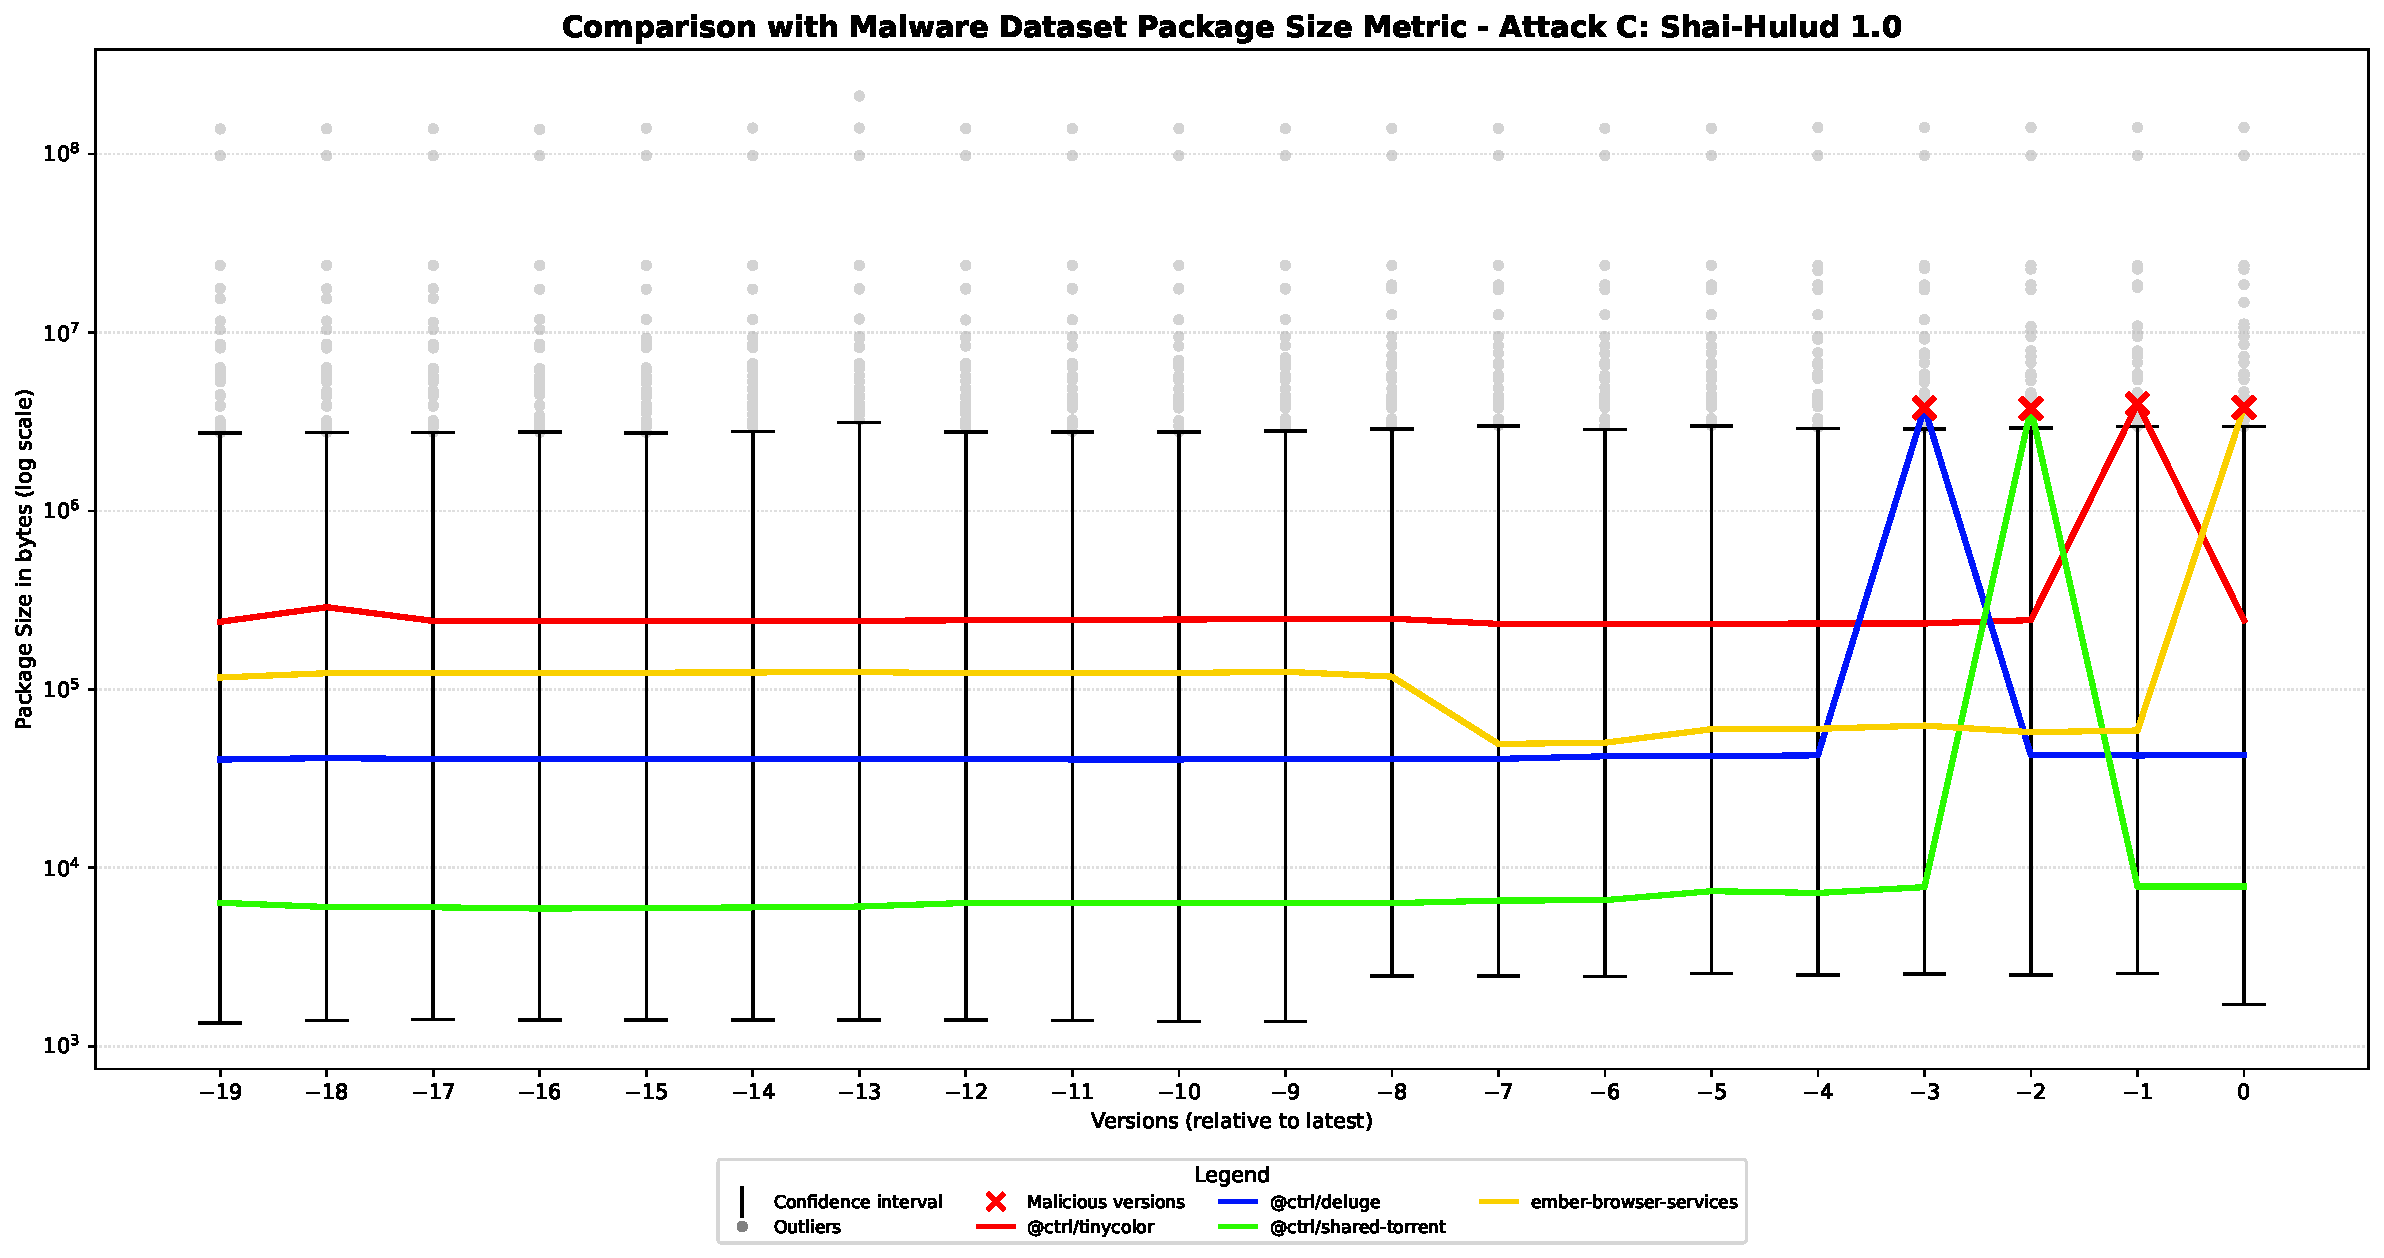
\includegraphics[width=\textwidth]{metrics/packageSize/PS_plot2single_AttackC.pdf}
    \caption{Comparison with Malware Dataset Package Size Metric for Attack C}
    \label{fig:fig2PackageSizeAttackC}
\end{figure}

Attack C (\cref{sec:attackC}) which adds a malicious file weighing approximately 3.7 MB,
succeeds in placing the compromised versions of the packages affected by this attack among the outlier values, 
as can be seen in \cref{fig:fig2PackageSizeAttackC}.
Therefore, the metric is effective for detecting this specific attack.

\subsection*{Attack D: Shai-Hulud 2.0}
\label{sec:analysisPackageSizeAttackD}

\begin{figure}[H]
    \centering
    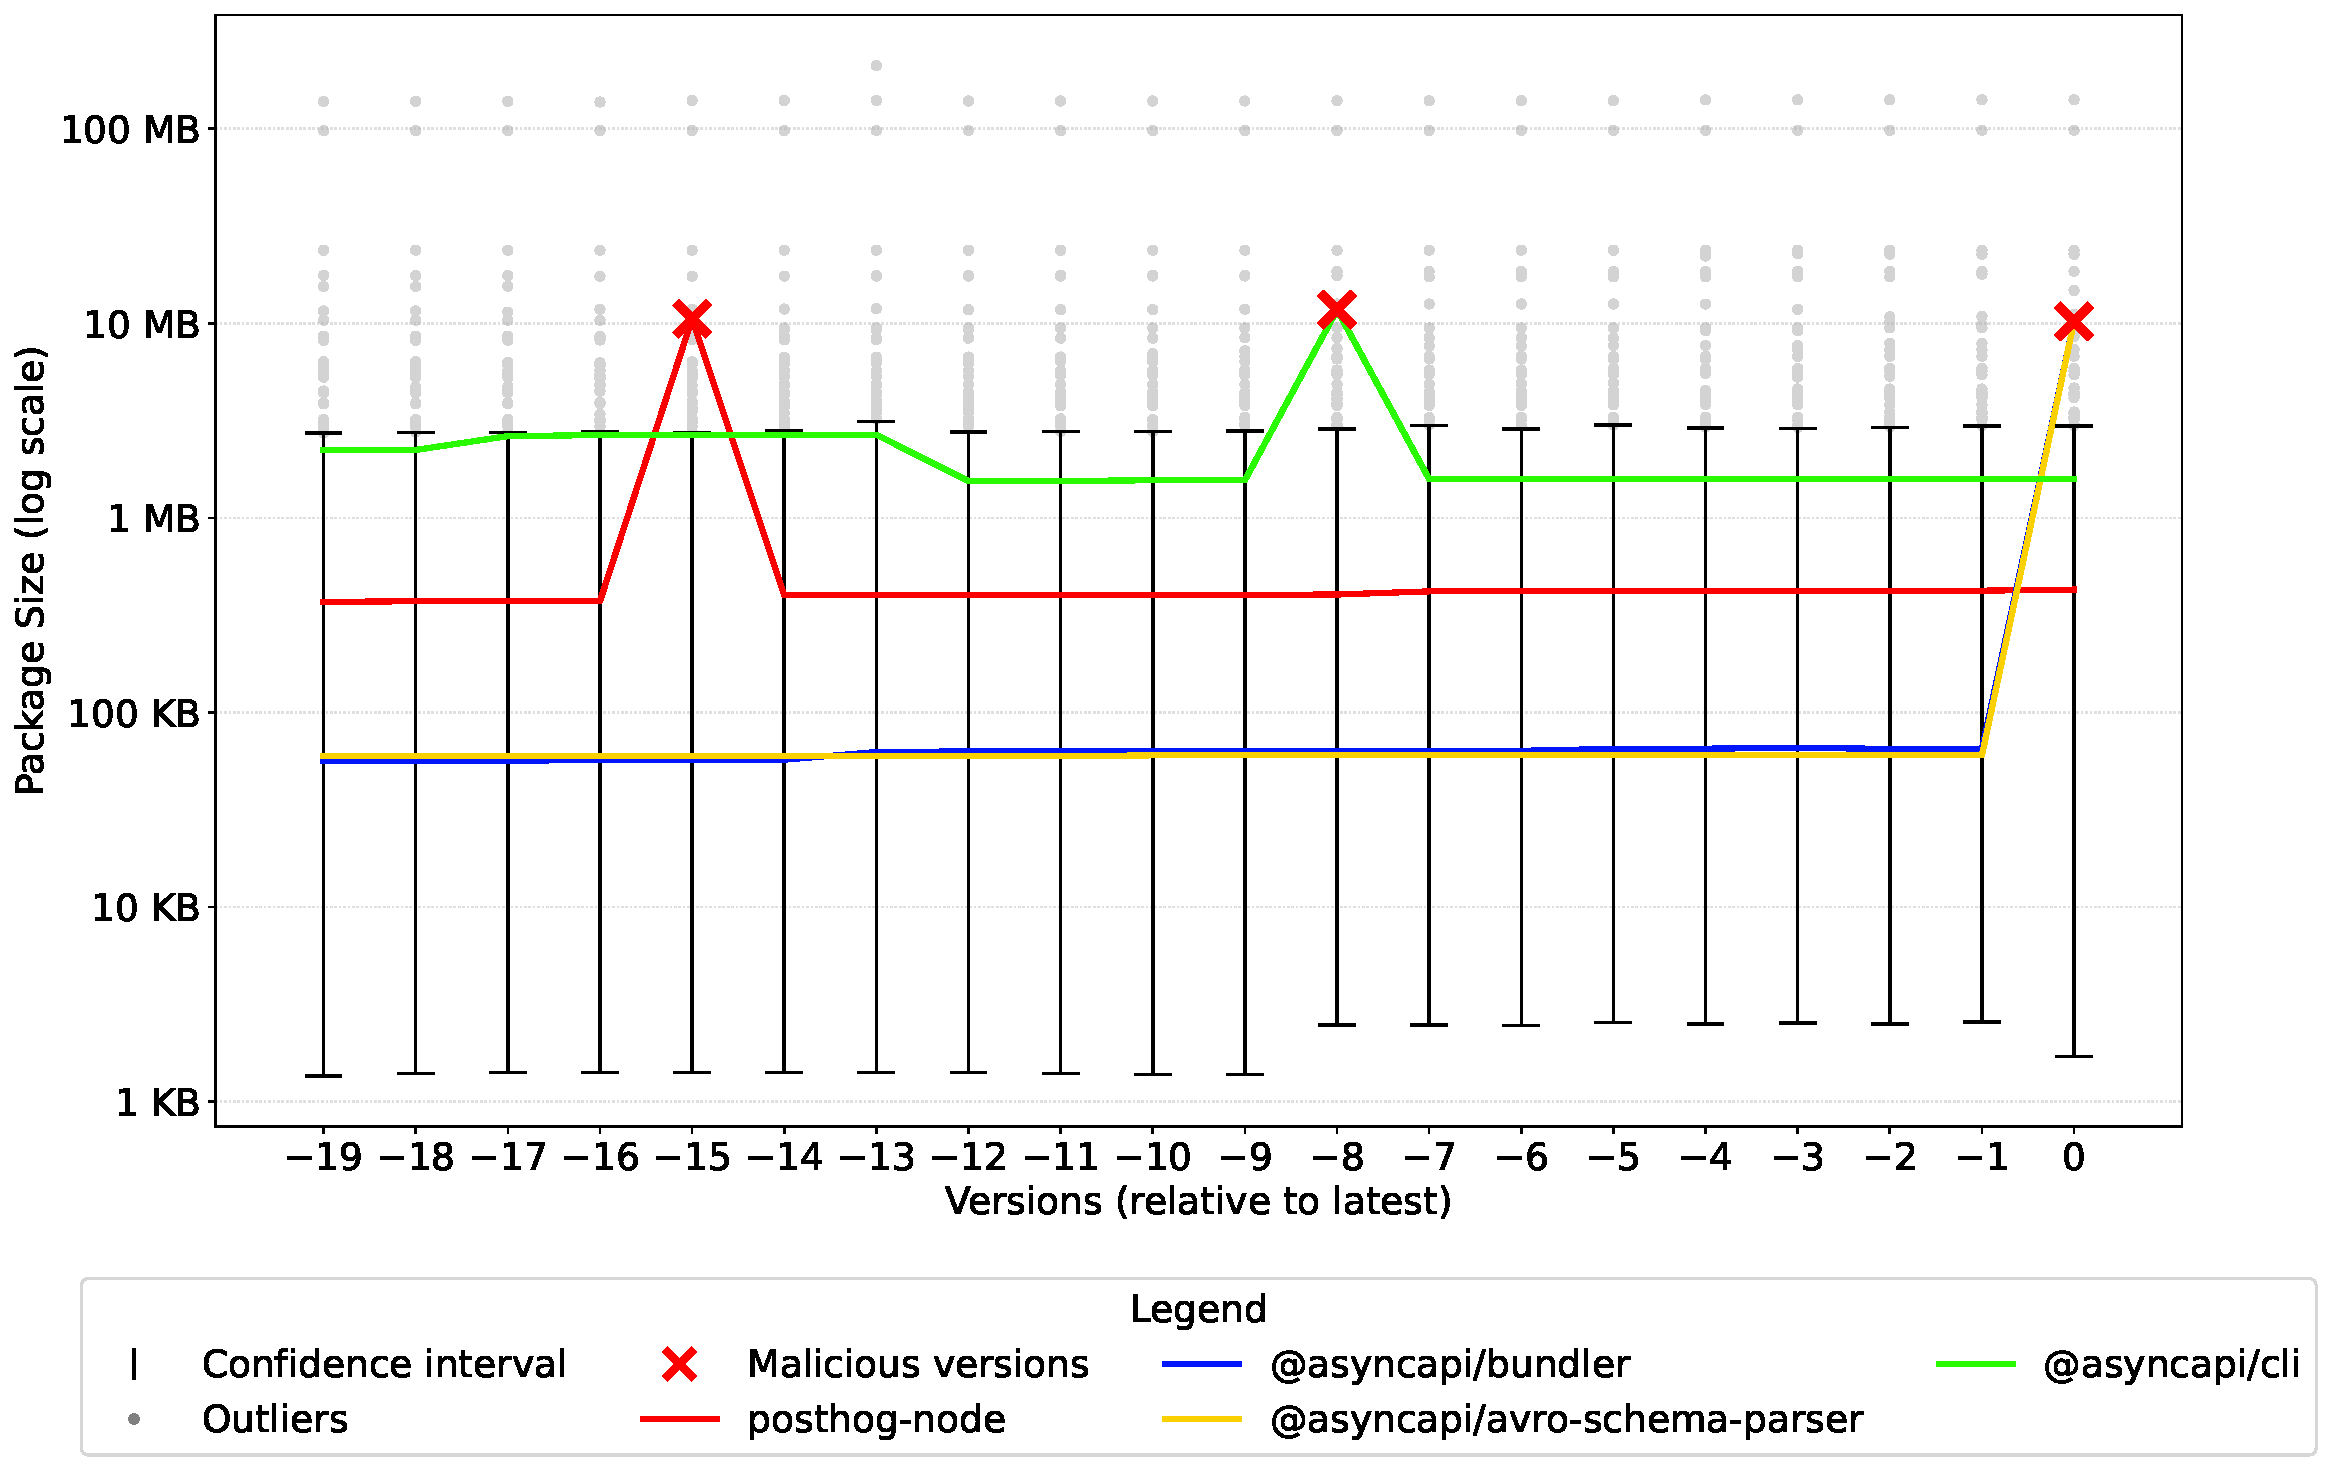
\includegraphics[width=\textwidth]{metrics/packageSize/PS_plot2single_AttackD.pdf}
    \caption{Comparison with Malware Dataset Package Size Metric for Attack D}
    \label{fig:fig2PackageSizeAttackD}
\end{figure}

Also for attack D (\cref{sec:attackD}) that introduces a malicious file weighing over 10 MB,
the metric is indicative for detecting this specific attack, as can be seen in \cref{fig:fig2PackageSizeAttackD}.

\subsection*{Summary of Comparison with Malware Dataset}
\label{sec:analysisPackageSizeSummaryComparisonMalware}

In summary, the metric is efficient in detecting the attack C (\texttt{Shai-Hulud}~1.0 \cref{sec:analysisPackageSizeAttackC}) 
and the attack D (\texttt{Shai-Hulud}~2.0 \cref{sec:analysisPackageSizeAttackD})
because, in both cases, the malicious versions have a package size that qualifies as outlier values.

Instead, the metric is not indicative for detecting the attack A (Malicious Windows DLL \cref{sec:analysisPackageSizeAttackA}) 
and the attack B (Crypto attack \cref{sec:analysisPackageSizeAttackB}) because, in both cases, 
the malicious versions have a package size that position them within the confidence intervals,
rendering them indistinguishable from legitimate versions.